\documentclass{ieeeaccess}
\usepackage{cite}
\usepackage{amsmath,amssymb,amsfonts}
\usepackage{algorithmic}
\usepackage{graphicx}
\usepackage{textcomp}
\usepackage{placeins}
\usepackage{afterpage}
\usepackage{float}

\def\BibTeX{{\rm B\kern-.05em{\sc i\kern-.025em b}\kern-.08em
    T\kern-.1667em\lower.7ex\hbox{E}\kern-.125emX}}
\begin{document}
\history{Date of publication xxxx 00, 0000, date of current version xxxx 00, 0000.}
\doi{10.1109/ACCESS.2017.DOI}

\title{AGENA: Kerangka Kerja AI Agen untuk Deteksi Iklan Native yang Dapat Dijelaskan pada Berita Digital}
\author{\uppercase{Brian Rizqi Paradisiaca Darnoto\authorrefmark{1,2}, Diana Purwitasari\authorrefmark{1,*}, \IEEEmembership{Senior Member, IEEE}, Daniel Siahaan\authorrefmark{1},\IEEEmembership{Member, IEEE}
}}
\address[]{\authorrefmark{1}Informatics Department, Institut Teknologi Sepuluh Nopember, Surabaya, 60111, Indonesia}
\address[]{\authorrefmark{2}Informatics, Universitas Jember, Jember, 68121, Indonesia}

\markboth
{Darnoto \headeretal: AGENA: Kerangka Kerja AI Agen}
{Darnoto \headeretal: AGENA: Kerangka Kerja AI Agen}

\corresp{Penulis korespondensi: Diana Purwitasari (e-mail: diana@its.ac.id).}

\begin{abstract}
Kebangkitan iklan \textit{native}, yang memadukan konten promosi dengan berita editorial, menimbulkan ancaman signifikan terhadap kredibilitas media digital dan kepercayaan pengguna. Meskipun model \textit{deep learning} tradisional telah menunjukkan hasil yang menjanjikan dalam mendeteksi konten semacam itu, model-model ini sering kali kurang memiliki transparansi dan kemampuan penjelasan (\textit{explainability}) yang diperlukan untuk aplikasi di ruang redaksi. Penelitian ini memperkenalkan AGENA, sebuah kerangka kerja AI agen (\textit{agentic AI}) canggih yang dirancang untuk deteksi dan penjelasan iklan \textit{native} secara otomatis di portal berita digital Indonesia. Berbeda dari arsitektur \textit{ensemble} statis, AGENA memperkenalkan kebaruan multi-dimensi dengan memanfaatkan \textit{pipeline} modular yang terdiri dari lima agen khusus: Web Scraper, Preprocessing, Retriever, Classifier, dan Explainer. Dengan memanfaatkan \textit{Retrieval-Augmented Generation} (RAG) dan \textit{Large Language Models} (LLM), kerangka kerja ini tidak hanya mengidentifikasi iklan \textit{native} dengan akurasi tinggi tetapi juga memberikan justifikasi yang dapat dibaca manusia atas klasifikasinya. Evaluasi eksperimental pada dataset berita Indonesia berskala besar menunjukkan bahwa pendekatan agen baru ini mencapai hasil \textit{state-of-the-art} sekaligus secara signifikan meningkatkan interpretabilitas model. Kerangka kerja ini menawarkan solusi yang kuat dan transparan bagi pemantau media dan konsumen berita, menjembatani kesenjangan antara deteksi otomatis dan penalaran yang berpusat pada manusia.
\end{abstract}

\begin{keywords}
AI Agen, AI yang Dapat Dijelaskan, LangChain, Iklan Native, Klasifikasi Berita, Retrieval-Augmented Generation.
\end{keywords}

\titlepgskip=-15pt

\maketitle

\section{Pendahuluan}
\label{sec:pendahuluan}
\textit{Native advertising} adalah konten media berbayar yang dirancang menyerupai gaya editorial platform tempat ia muncul \cite{b1}. Tidak seperti format iklan konvensional seperti spanduk atau \textit{interstitial}, iklan \textit{native} terintegrasi ke dalam halaman berita sehingga sulit dikenali sebagai konten komersial oleh pembaca \cite{b2}. Meskipun format ini menguntungkan pengiklan dari sisi keterlibatan pengguna \cite{b3}, ia juga menimbulkan kekhawatiran serius terkait kemandirian editorial dan transparansi konten jurnalistik \cite{b4}.

Dalam lanskap berita digital Indonesia, iklan \textit{native} sangat lazim ditemukan. Portal-portal dengan trafik tinggi seperti Kompas, Detik, dan Tempo secara rutin menerbitkan konten yang memenuhi tujuan promosi sambil mempertahankan gaya berita organik \cite{b5}. Ketiadaan praktik pengungkapan yang terstandarisasi menimbulkan kekhawatiran terhadap transparansi dan kepercayaan publik \cite{b6}. Dari sudut pandang analitis, konten seperti ini merupakan bentuk penipuan kontekstual, di mana otoritas jurnalistik dimanfaatkan untuk secara implisit mendorong klaim komersial \cite{b7}. Deteksi otomatis atas konten semacam ini merupakan persoalan penting bagi pengawasan media.

Mendeteksi iklan \textit{native} lebih kompleks dibandingkan mengidentifikasi propaganda atau misinformasi faktual. Yang terakhir biasanya bergantung pada klaim palsu \cite{b8}, sementara iklan \textit{native} sering kali akurat secara faktual namun dibingkai secara strategis. Efek persuasifnya berasal dari penggunaan bahasa promosi yang selektif: hiperbola halus, ketiadaan sudut pandang kritis, dan penekanan pada pencapaian perusahaan yang disajikan sebagai berita \cite{b9}. Dalam konteks Indonesia, tantangan ini diperumit oleh keberagaman gaya penulisan regional dan penggunaan idiom informal yang mempersulit analisis linguistik otomatis. Pada volume konten yang dihasilkan oleh portal berita besar per harinya, tinjauan manual tidak memungkinkan \cite{b10}.

Kemajuan terkini pada \textit{Large Language Models} (LLM) membuka kemungkinan baru untuk klasifikasi teks yang bernuansa. Model seperti Qwen \cite{b11}, Llama \cite{b12}, GPT-4o \cite{b13}, dan keluarga Gemma \cite{b14} telah menunjukkan performa yang kompetitif pada tugas-tugas NLP Indonesia ketika dikombinasikan dengan pendekatan berbasis \textit{retrieval} \cite{b15}. Namun demikian, penerapan model-model ini secara langsung pada deteksi iklan \textit{native} mengungkap dua kelemahan yang konsisten. Pertama, LLM standar menghasilkan label biner tanpa menjelaskan alasan di balik keputusannya, membatasi kegunaannya dalam alur kerja ruang redaksi. Kedua, model ini rentan terhadap halusinasi ketika menghadapi pola bahasa spesifik domain yang kurang terwakili dalam data pra-pelatihan \cite{b16}. Kerangka kerja yang menggabungkan kapasitas penalaran LLM dengan landasan domain dan keluaran yang dapat diinterpretasi oleh manusia menjadi kebutuhan yang mendesak.

Penelitian sebelumnya tentang deteksi iklan \textit{native}, termasuk kerangka kerja SENADA, mengandalkan pengklasifikasi \textit{stacked ensemble} yang memecah tugas deteksi ke dalam sub-model independen untuk sentimen, persuasi, promosi, dan perspektif \cite{b17, b18, b19}. Pendekatan ini menetapkan tolok ukur performa yang kuat, namun tidak memiliki interpretabilitas dan tidak dapat menghasilkan justifikasi yang dapat ditinjau oleh editor \cite{b20}. Ini adalah keterbatasan signifikan di lapangan, karena pengawasan editorial membutuhkan tidak hanya keputusan, tetapi juga penjelasan mengapa suatu konten ditandai. Kesenjangan interpretabilitas ini telah diakui dalam studi-studi sebelumnya mengenai deteksi konten persuasif pada berita Indonesia \cite{b21}.

Makalah ini memperkenalkan AGENA (\textit{Agentic AI Framework for Explainable Native Advertisement Detection}), sebuah sistem multi-agen yang mengatasi kesenjangan tersebut. AGENA memecah tugas deteksi ke dalam sebuah \textit{pipeline} berurutan dari lima agen khusus: (1) \textit{Web Scraper} untuk ekstraksi konten, (2) \textit{Preprocessor} untuk rekayasa fitur linguistik, (3) \textit{Retriever} untuk landasan konteks berbasis RAG, (4) \textit{Classifier} untuk penalaran rantai-pemikiran, dan (5) \textit{Explainer} untuk menghasilkan justifikasi yang dapat diaudit.

Kontribusi utama penelitian ini adalah:
\begin{enumerate}
    \item \textbf{Kontribusi arsitektural}: Kami mengusulkan \textit{pipeline} AGENA, sebuah sistem lima agen untuk deteksi iklan \textit{native} pada berita digital Indonesia. Sejauh pengetahuan kami, ini adalah kerangka kerja deteksi multi-agen pertama yang didedikasikan untuk domain ini.
    \item \textbf{Kontribusi metodologis}: Kami memperkenalkan strategi \textit{fine-tuning} ``\textit{Reasoning-First}'' yang dilandasi RAG, terikat pada basis pengetahuan yang terdiri dari 12.088 artikel berita Indonesia. Pendekatan ini mengurangi halusinasi dan meningkatkan diskriminasi kasus ``\textit{Hard Negative}''.
    \item \textbf{Kontribusi evaluatif}: Kami mengevaluasi kualitas keluaran model melampaui metrik akurasi menggunakan protokol ``\textit{LLM-as-a-Judge}'', di mana GPT-4o menilai jejak penalaran pada skala 1--5 berdasarkan empat kriteria interpretabilitas: keselarasan Sentimen, Persuasi, Promosi, dan Perspektif.
\end{enumerate}

Sisa dari makalah ini diatur sebagai berikut. Bagian \ref{sec:related-works} mengulas pekerjaan terkait pada \textit{machine learning}, LLM, dan AI agen untuk analisis media. Bagian \ref{sec:dataset} mendeskripsikan dataset. Bagian \ref{sec:methods} menyajikan arsitektur dan algoritma AGENA. Bagian \ref{sec:experiments} melaporkan hasil eksperimen. Bagian \ref{sec:discussion} dan \ref{sec:conclusion} membahas implikasi dan kesimpulan.



\section{Pekerjaan Terkait}
\label{sec:related-works}
Kami membahas penelitian terdahulu dari tiga area yang relevan dengan AGENA: \textit{machine learning} untuk deteksi iklan, model bahasa besar dengan augmentasi retrieval, dan sistem AI agen.

\subsection{Machine Learning dan Deep Learning dalam Deteksi Iklan}
Pendekatan awal untuk deteksi iklan \textit{native} otomatis mengandalkan fitur yang dibuat secara manual seperti rasio kapitalisasi, frekuensi kata kunci, dan panjang kalimat untuk melatih pengklasifikasi termasuk SVM dan Naive Bayes \cite{b3}. Meski metode ini menetapkan tolok ukur awal, kemampuannya tidak memadai untuk memodelkan kompleksitas linguistik konten promosi modern.

Pendekatan \textit{deep learning} memperbaiki hal ini dengan memungkinkan ekstraksi fitur otomatis. Arsitektur CNN diaplikasikan untuk mendeteksi pola semantik lokal, sementara jaringan LSTM menangkap ketergantungan naratif jangka panjang \cite{b22}. Sistem yang patut dicatat dalam area ini adalah SENADA, yang memecah tugas deteksi ke dalam empat sub-model \textit{ensemble} yang selaras dengan dimensi teoritis persuasi (Sentimen, Persuasi, Promosi, Perspektif) \cite{b17}. Meski hasilnya kuat, model-model tersebut tidak menghasilkan keluaran eksplanatori, sehingga membatasi adopsinya di lingkungan editorial yang menuntut transparansi keputusan.

\subsection{Large Language Models dan Retrieval-Augmented Generation}
Arsitektur Transformer \cite{b23} menetapkan standar baru untuk tugas klasifikasi teks. BERT dan variannya (RoBERTa, T5) menunjukkan bahwa pemodelan konteks dua arah secara substansial meningkatkan performa pada deteksi propaganda dan misinformasi \cite{b8}, \cite{b9}. Dalam domain berita, LLM telah digunakan untuk menilai netralitas konten dan memeriksa bias pemangku kepentingan \cite{b24}.

Keterbatasan yang berulang dari LLM yang berdiri sendiri adalah halusinasi domain-spesifik. \textit{Retrieval-Augmented Generation} (RAG) mengatasi hal ini dengan menggabungkan model inferensi dengan basis data vektor (mis., FAISS, Pinecone), memungkinkan model untuk mengambil dan mengkondisikan penalaran pada contoh-contoh relevan yang ada sebelumnya \cite{b25}, \cite{b26}. Desain ini sangat berguna untuk tugas pemantauan berita, di mana contoh-contoh historis yang diambil berfungsi sebagai bukti landasan untuk mengklasifikasikan artikel baru \cite{b27}, \cite{b16}. Namun, sebagian besar sistem RAG yang ada beroperasi sebagai \textit{pipeline} retrieval satu langkah dan tidak mendukung pengambilan keputusan multi-langkah yang otonom.

\subsection{Kemunculan AI Agen dan Sistem Multi-Agen}
\textit{Agentic AI} mengacu pada sistem di mana LLM berfungsi sebagai mesin penalaran otonom yang mampu merencanakan, menggunakan alat, dan melakukan eksekusi multi-langkah \cite{b10}, \cite{b28}. Kerangka kerja orkestrasi seperti LangChain dan AutoGen memungkinkan komposisi LLM dengan alat pencarian, API, dan modul memori ke dalam \textit{pipeline} terstruktur \cite{b29}, \cite{b30}.

Sistem agen telah diterapkan dengan efektivitas yang cukup baik dalam tugas-tugas yang memerlukan verifikasi multi-langkah, termasuk deteksi misinformasi dan audit bias politik \cite{b31, b32}. Untuk jurnalisme digital Indonesia khususnya, pendekatan agen sangat cocok karena dapat menggabungkan alat khusus bahasa dan basis pengetahuan regional-spesifik yang tidak akan ditangkap oleh pengklasifikasi generik. Ini membangun landasan dari penelitian sebelumnya tentang NLP sumber daya rendah untuk bahasa Indonesia \cite{b33} dan klasifikasi multi-label konten berbasis ucapan \cite{b34}. Penyertaan Agen Penjelasan yang berdedikasi juga mengatasi persyaratan interpretabilitas yang diakui dalam studi adopsi ruang redaksi sebelumnya \cite{b20}. AGENA memperluas jalur penelitian ini dengan menyediakan \textit{pipeline} multi-agen pertama yang didedikasikan untuk deteksi iklan \textit{native} dalam berita Indonesia, dengan penekanan pada akurasi klasifikasi, transparansi penalaran, dan orkestrasi berbasis grafik \cite{b35}.

\section{Dataset}
\label{sec:dataset}
Fondasi dari penelitian ini adalah kumpulan dataset ekstensif dari artikel berita elektronik berbahasa Indonesia, yang dikurasi secara khusus untuk deteksi iklan \textit{native} \cite{b17}. Dataset ini terdiri dari 12.088 artikel yang dikumpulkan dari enam portal berita Indonesia utama (misalnya, Kompas, Detik, Tempo) antara bulan Februari dan Agustus 2022. Koleksi ini mencakup berbagai kategori sesuai yang diringkas pada Tabel \ref{tab:dataset_stats}.

\begin{table}[htbp]
\caption{Distribusi Dataset di Berbagai Kategori Berita}
\label{tab:dataset_stats}
\begin{center}
\begin{tabular}{|l|c|c|c|}
\hline
\textbf{Kategori} & \textbf{Total Artikel} & \textbf{Iklan Native} & \textbf{Berita Murni} \\
\hline
Ekonomi & 1.914 & 1.349 & 565 \\
Gaya Hidup & 1.807 & 415 & 1.392 \\
Hiburan & 635 & 128 & 507 \\
Internasional & 359 & 90 & 269 \\
Nasional & 1.262 & 595 & 667 \\
Lainnya & 3.565 & 2.882 & 683 \\
Otomotif & 474 & 106 & 368 \\
Pendidikan & 274 & 70 & 204 \\
Olahraga & 823 & 69 & 754 \\
Teknologi & 975 & 340 & 635 \\
\hline
\textbf{Total} & \textbf{12.088} & \textbf{5.944} & \textbf{6.144} \\
\hline
\end{tabular}
\end{center}
\end{table}

Aspek penting dari dataset ini adalah anotasi multi-labelnya. Setiap artikel dianotasi secara manual oleh tiga ahli independen berdasarkan empat karakteristik implisit: (1) sentimen positif atau netral, (2) nada persuasif, (3) fokus promosi, dan (4) perspektif sumber tunggal. Kesepakatan antar-anotator, yang diukur melalui \textit{Fleiss' Kappa}, mencapai 0,90, yang mengindikasikan reliabilitas tinggi. Dalam AGENA, dataset ini memiliki tujuan ganda: dataset ini digunakan untuk melatih sistem (\textit{fine-tuning}) LLM yang mendasarinya dan bertindak sebagai basis pengetahuan pokok (\textit{ground-truth}) untuk komponen RAG, kemudian disimpan dalam ruang vektor berdimensi tinggi (\textit{high-dimensional vector space}) untuk pengambilan konteks secara \textit{real-time}.

\section{Metode yang Diusulkan}
\label{sec:methods}
Kerangka kerja AGENA (\textit{Agentic Native Ads detection}) dikonseptualisasikan sebagai sistem multi-agen terdistribusi yang menggeser paradigma deteksi dari peristiwa klasifikasi tunggal menjadi proses penalaran kolaboratif multi-tahap. Arsitektur ini dilandaskan pada prinsip "Reasoning-First" (Penalaran-Dahulu), di mana pembuatan bukti interpretatif diperlakukan sebagai prekursor penting sebelum pemberian label klasifikasi final.

\subsection{Fondasi Filosofis: Paradigma Reasoning-First}
Pengklasifikasi berita tradisional beroperasi sebagai model diskriminatif yang memetakan masukan $X$ secara langsung ke label $Y$. Meski efisien, pendekatan ini tidak memberikan wawasan mengenai "mengapa" secara linguistik di balik suatu keputusan. AGENA mengadopsi pendekatan penalaran generatif di mana model harus terlebih dahulu menyusun jejak penalaran multi-dimensi $T$. Jejak ini bertindak sebagai jembatan semantik, memetakan kembali fitur-fitur artikel ke karakteristik teoritis iklan \textit{native}. Dengan memaksa model untuk mengartikulasikan penemuannya sebelum menentukan label, kita secara signifikan memitigasi risiko halusinasi stokastik dan meningkatkan presisi klasifikasi.

\subsection{Definisi Formal dan Manajemen Status}
Kami mendefinisikan sistem AGENA bukan sebagai lintasan linier tunggal, melainkan sebagai sistem transisi status siklik nan dinamis yang ditenagai oleh \texttt{StateGraph} dari LangChain. Misalkan $S_{state}$ adalah kamus status global (\textit{state dictionary}) yang bertindak sebagai penyangga memori (\textit{memory buffer}) untuk seluruh rangkaian deteksi. Ruang status didefinisikan oleh skema berikut:
\begin{equation}
S_{state} = \{U, D, F, K, R\}
\end{equation}
di mana $U$ mewakili URL target, $D$ adalah teks dokumen mentah yang diekstraksi, $F$ adalah vektor fitur sintaksis dan semantik, $K$ adalah konteks yang diperkaya untuk kebutuhan pengambilan (\textit{retrieved augmented context}), dan $R$ adalah hasil penalaran akhir yang berisi prediksi Boolean sekaligus jejak penjelasan.

Kerangka kerja ini mencakup lima agen otonom $A = \{A_{scrape}, A_{prep}, A_{ret}, A_{class}, A_{exp}\}$ yang membaca dan memutasi nilai $S_{state}$ secara asinkron:
\begin{itemize}
    \item \textbf{Scraper Agent ($A_{scrape}$)}: Mengeksekusi mutasi status $\delta_{scrape}: S_{state}[U] \rightarrow S_{state}[D]$. Ia memanfaatkan \textit{headless browser} untuk memastikan perenderan fidelitas tinggi (\textit{high-fidelity rendering}) dari simpul DOM yang dinamis sebelum menuliskan dokumen $D$ yang bersih ke dalam status.
    \item \textbf{Preprocessing Agent ($A_{prep}$)}: Mengeksekusi $\delta_{prep}: S_{state}[D] \rightarrow S_{state}[F]$. Agen ini memproses $D$ untuk mengekstraksi fitur sintaksis berdimensi-$n$ (misalnya, jumlah hiperbola, densitas huruf kapital) dan penanda semantik.
    \item \textbf{Retriever Agent ($A_{ret}$)}: Mengeksekusi $\delta_{ret}: (S_{state}[D], \mathcal{MB}) \rightarrow S_{state}[K]$. Ia menghitung nilai kemiripan kosinus terhadap penyangga memori (\textit{memory buffer}) $\mathcal{MB}$ berindeks FAISS (yang menampung 12.088 artikel dasar) dan menuliskan jangkar kontekstual top-$k$ kembali ke dalam $K$.
    \item \textbf{Classifier Agent ($A_{class}$)}: Melaksanakan logika evaluatif inti $\delta_{class}: (S_{state}[D], S_{state}[F], S_{state}[K]) \rightarrow L$, di mana $L \in \{0, 1\}$ mewakili klasifikasi Boolean tahap awal berdasarkan integrasi keseluruhan data status.
    \item \textbf{Explainer Agent ($A_{exp}$)}: Mengeksekusi $\delta_{exp}: (S_{state}[D], S_{state}[K], L) \rightarrow S_{state}[R]$. Ia membangun jejak justifikasi yang dapat dibaca manusia (\textit{human-readable justification trace}), memetakan alur logis kembali ke rukun inti kaidah jurnalisme \textit{native}.
\end{itemize}

\subsection{Orkestrasi Agen Hierarkis}
Tidak seperti \textit{pipeline} linier tradisional, interaksi antar agen dalam AGENA diatur oleh grafik berstatus (\textit{stateful graph}). Orkestrator mengelola "\textit{Agentic Context Buffer}" yang mengumpulkan gradien informasi dari setiap titik.

\subsection{Kumpulan Alat Agen dan Logika Keputusan yang Merinci}
Setiap agen dalam ekosistem AGENA dilengkapi dengan seperangkat alat khusus:

\subsubsection{Web Scraper Agent}
Agen ini memanfaatkan alat \texttt{Web\allowbreak Scraper\allowbreak Tool} dan \texttt{Selenium\allowbreak Scraper\allowbreak Tool}, menggabungkan \texttt{Beautiful\allowbreak Soup4} untuk struktur DOM statis dan \texttt{Selenium} untuk konten dinamis. Agen ini mengimplementasikan logika "pembersih" otomatis yang menghapus \textit{boilerplate} non-jurnalistik (misalnya, \textit{footer}, iklan di dalam iklan, bilah navigasi) untuk memastikan bahwa Classifier hanya memproses batang tubuh narasi inti.

\subsubsection{Preprocessing Agent}
Logika prapemrosesan (\textit{preprocessing}) melampaui pembersihan standar. Agen ini memanfaatkan pendekatan hibrida:
\begin{enumerate}
    \item \textbf{Normalisasi Teks}: Menghapus karakter yang tidak relevan, URL, dan menstandardisasi spasi putih menggunakan Regex.
    \item \textbf{Ekstraksi Fitur}: Menggunakan ekspresi reguler dan \textit{array} statistik (\texttt{numpy}) untuk mengekstraksi fitur seperti panjang teks, jumlah kata unik, keragaman leksikal, dan rasio huruf kapital.
\end{enumerate}

\subsubsection{Retriever Agent}
\textit{Retriever Agent} mengimplementasikan strategi pencarian semantik menggunakan indeks FAISS (\textit{Facebook AI Similarity Search}). Proses pengambilan ini dirumuskan dalam Algoritma 1. Agen ini menghitung kemiripan kosinus (\textit{cosine similarity}) antara sematan (\textit{embedding}) artikel saat ini $\vec{v}_D$ dan sematan dalam basis pengetahuan $\vec{v}_K$. Jangkar (\textit{anchors}) top-K berfungsi sebagai titik pembelajaran dalam-konteks (\textit{in-context learning}/ICL) \textit{few-shot} untuk \textit{Classifier}.

\subsubsection{Classifier Agent}
Agen ini adalah "pengendali" dari proses penalaran. Agen ini dibangun di atas model Qwen 2.5 14B yang telah di-\textit{fine-tune}, dioptimalkan untuk nuansa jurnalistik Indonesia. Batas keputusan agen dibentuk oleh \textit{prompt} hierarkis yang mencakup lapisan metakognitif (mendefinisikan "persona"), lapisan domain (standar editorial berita), dan lapisan batasan (skema keluaran).

\subsubsection{Explanation Agent}
Agen ini beroperasi sebagai pasca-pemroses (\textit{post-processor}) untuk keluaran LLM. Agen ini memanfaatkan alat \texttt{Source\allowbreak Mapper} untuk menautkan klaim penalaran spesifik kembali ke cuplikan teks asli. Misalnya, jika \textit{Classifier} mengidentifikasi "Penyebutan merek yang berlebihan", \textit{Explanation Agent} memindai teks untuk memberikan frekuensi dan lokasi yang tepat dari nama merek tersebut, memberikan verifikasi empiris untuk klaim model asalnya.

\subsection{Kedalaman Algoritmik}
Logika operasional inti untuk penalaran berlandaskan RAG disajikan dalam Algoritma 1, sementara strategi penyelarasan "Reasoning-First" yang khusus didefinisikan dalam Algoritma 2.

\begin{algorithmic}
\STATE \textbf{Algoritma 1: Klasifikasi Agenik dengan RAG}
\REQUIRE Artikel Mentah $D$, Vektor KB $K$
\ENSURE Label Klasifikasi $L$, Jejak Penalaran $T$
\STATE $D^* \leftarrow S.Extract(D)$ \COMMENT{Ekstraksi akurasi tinggi}
\STATE $F \leftarrow P.distill(D^*)$ \COMMENT{Rekayasa fitur sintaksis}
\STATE $Context \leftarrow R.search(D^*, K, k=5)$ \COMMENT{Penjangkaran semantik}
\STATE $T, L \leftarrow C.reason(D^*, F, Context)$ \COMMENT{Eksekusi Reasoning-First}
\RETURN $L, T$
\end{algorithmic}

\begin{algorithmic}
\STATE \textbf{Algoritma 2: Penyelarasan Prompt Reasoning-First}
\REQUIRE Input $X$, Karakteristik $C_{markers}$, Contoh $E_{shots}$
\ENSURE Jejak Selaras $T$
\STATE Tentukan Identitas Sistem $I \leftarrow \text{"Senior News Editor"}$
\FOR{setiap $m \in C_{markers}$}
    \STATE $Step_m \leftarrow \text{Analisis } X \text{ untuk karakteristik } m$
\ENDFOR
\STATE $Context \leftarrow \text{Agregat } (Step_m)$
\STATE $T \leftarrow \text{SynthesizeContext}(I, Context, E_{shots})$
\RETURN $T$
\end{algorithmic}

\subsection{Rekayasa Prompt dan Penyelarasan Few-Shot}
Untuk memastikan akurasi klasifikasi yang tinggi (97\%) dan meminimalkan halusinasi, AGENA memanfaatkan \textit{prompt} sistem "Reasoning-First". Tidak seperti klasifikasi \textit{zero-shot} standar, \textit{Classifier Agent} diinstruksikan untuk melakukan analisis rantai-pemikiran (\textit{chain-of-thought}) sebelum mengeluarkan label akhir. Struktur \textit{prompt} didefinisikan sebagai berikut:

\begin{itemize}
    \item \textbf{Identitas Sistem}: Mendefinisikan agen sebagai editor senior dengan keahlian mendeteksi niat komersial yang tersembunyi.
    \item \textbf{Penjangkaran Karakteristik}: Memaksa agen untuk mengevaluasi teks terhadap empat penanda teoritis (Sentimen, Persuasi, Promosi, Perspektif).
    \item \textbf{Injeksi Kontekstual}: Menuntikkan top-5 artikel yang paling mirip yang diambil sebagai penanda batas semantik.
    \item \textbf{Batasan Respons}: Menerapkan skema JSON khusus untuk memfasilitasi penguraian terprogram dan pemetaan penjelasan di hilir.
\end{itemize}

Mesin penalaran inti (Qwen, Gemma, Llama, dan GPT-4o) yang digunakan dalam kerangka kerja AGENA dioptimalkan untuk peran khusus. Setiap model memiliki peran spesifik, baik sebagai agen pengklasifikasi utama maupun sebagai hakim evaluasi.

Sebuah contoh dari templat \textit{few-shot} yang digunakan saat melatih (fine-tuning) model Qwen 2.5 14B disediakan dalam materi pelengkap, yang memastikan bahwa model mempelajari perbedaan bernuansa khusus antara "pelaporan positif" dan "bias promosi".

\subsection{Penyetelan Model dan Hyperparameter}
Mesin penalaran inti (Qwen, Gemma, Llama) dilatih ulang menggunakan teknik \textit{Parameter-Efficient Fine-Tuning} (PEFT), secara spesifik \textit{Low-Rank Adaptation} (LoRA) \cite{b36} dan kuantisasi 4-bit (QLoRA). Pendekatan ini memungkinkan optimalisasi model berskala besar di dalam batasan memori GPU yang tersedia. \textit{Hyperparameter} spesifik yang digunakan dalam proses \textit{fine-tuning} dirinci dalam Tabel \ref{tab:hyperparameters}.

\begin{table*}[htbp]
\caption{Hyperparameter Fine-tuning di Berbagai Model}
\label{tab:hyperparameters}
\begin{center}
\begin{tabular}{|l|c|c|c|}
\hline
\textbf{Hyperparameter} & \textbf{Qwen 14B} & \textbf{Gemma 9B} & \textbf{Llama 8B} \\
\hline
Peringkat LoRA (\textit{Rank} $r$) & 32 & 16 & 16 \\
LoRA Alpha ($\alpha$) & 64 & 32 & 32 \\
Laju Pembelajaran (\textit{Learning Rate}) & 2e-5 & 5e-5 & 3e-5 \\
Ukuran Batch (\textit{Batch Size}) & 16 & 8 & 8 \\
Epos (\textit{Epochs}) & 3 & 5 & 5 \\
Kuantisasi & 4-bit & 4-bit & 4-bit \\
Pengoptimal (\textit{Optimizer}) & AdamW & AdamW & AdamW \\
\hline
\end{tabular}
\end{center}
\end{table*}

\subsection{Kerangka Kerja Evaluasi LLM-as-a-Judge}
Untuk mengevaluasi kedalaman kualitatif dari keluaran \textit{Explainer Agent}, AGENA menggunakan metodologi "LLM-as-a-Judge". Model terdepan (\textit{frontier model}, yaitu GPT-4o-mini) bertindak sebagai editor ahli untuk menilai jejak penalaran pada skala kontinu 1 hingga 5. Templat \textit{prompt} hakim menetapkan tiga kriteria evaluasi yang ketat:
\begin{enumerate}
    \item \textbf{Akurasi Label}: Kebenaran menurut \textit{ground truth} yang dianotasi manusia.
    \item \textbf{Kualitas Penalaran}: Koherensi logis yang menghubungkan prediksi dengan sifat-sifat naratif tertentu (mis., nada promosi versus pelaporan obyektif).
    \item \textbf{Pemeriksaan Hard Negative}: Kemampuan untuk mengklasifikasikan secara akurat berita editorial yang banyak menyebutkan entitas perusahaan tanpa secara bawaan mempromosikannya.
\end{enumerate}
Dimensi kualitatif ini melengkapi metrik biner standar (Akurasi, F1-Score) dengan memberi penalti pada model yang mencapai label benar melalui penalaran yang berhalusinasi atau dangkal.

Strategi \textit{tuning} "Reasoning-First" melibatkan penambahan penalaran \textit{Chain-of-Thought} sebelum label target di dalam dataset pelatihan. Hal ini memaksa model untuk mempelajari langkah-langkah perantara linguistik (misal, mengidentifikasi penanda persuasif, mendeteksi bias sumber) sebelum menentukan label klasifikasi akhir. Kami memanfaatkan FlashAttention-2 \cite{b37} untuk mengakselerasi komputasi \textit{self-attention}, yang memungkinkan konvergensi lebih cepat.
Performa kerangka kerja AGENA dievaluasi melalui serangkaian eksperimen yang berfokus pada akurasi klasifikasi, kualitas penalaran, dan dampak dari komponen \textit{Retrieval-Augmented Generation} (RAG).

\section{Eksperimen dan Hasil}
\label{sec:experiments}
\subsection{Penyiapan Eksperimental}
Eksperimen dilakukan menggunakan dataset berita Indonesia yang terdiri dari 12.088 artikel. Komponen LLM (\textit{Classifier} dan \textit{Explainer}) dilatih ulang menggunakan kerangka kerja Unsloth dengan adaptor LoRA (\textit{Rank}=16, \textit{Alpha}=32). Pelatihan dilakukan pada infrastruktur komputasi kinerja tinggi. Dataset dibagi menjadi set pelatihan dan pengujian, dengan set pengujian mencakup beragam sampel "Hard Negatives" untuk mengevaluasi ketahanan model.

\subsection{Performa Kuantitatif}
Tabel \ref{tab:detailed_comparison} merangkum performa berbagai \textit{Large Language Models} yang diintegrasikan sebagai mesin penalaran inti dalam \textit{pipeline} AGENA.

\subsection{Rincian Performa Kuantitatif}
Performa \textit{pipeline} AGENA dievaluasi di beberapa iterasi \textit{fine-tuning} model, secara khusus membandingkan \textit{Instruction Tuning} standar terhadap Strategi Prompt "Reasoning-First" yang diusulkan. Kerangka kerja ini mengimplementasikan pemformatan dataset bersyarat: menetapkan Prompt Reasoning-First Dasar untuk arsitektur yang lebih kecil seperti Gemma-3 (270M), dan Prompt JSON Reasoning-First untuk model berukuran lebih besar (Qwen 14B, Gemma 3 12B, Llama 8B, Gemma 9B).

\begin{table}[htbp]
\caption{Metrik Performa untuk LLM Dasar}
\label{tab:detailed_comparison}
\begin{center}
\begin{tabular}{|l|c|c|c|c|}
\hline
\textbf{Model} & \textbf{Recall} & \textbf{Precision} & \textbf{F1-score} & \textbf{Akurasi} \\
\hline
Gemma 3 (12B) & 0,948 & 0,938 & 0,943 & 94,50\% \\
Gemma 3 (4B) & 0,927 & 0,908 & 0,918 & 92,00\% \\
Gemma 2 (9B) & 0,958 & 0,860 & 0,906 & 90,50\% \\
Gemma 3 (1B) & 0,979 & 0,676 & 0,800 & 76,50\% \\
Qwen 2.5 (14B) & 0,958 & 0,635 & 0,764 & 71,50\% \\
Llama 3.1 (8B) & 0,792 & 0,571 & 0,664 & 61,50\% \\
GPT-OSS & 0,833 & 0,541 & 0,656 & 57,50\% \\
Gemma 3 (270M) & 0,520 & 0,547 & 0,480 & 52,00\% \\
\hline
\end{tabular}
\end{center}
\end{table}

Hasil dari penyelarasan \textit{prompt} ``\textit{Reasoning-First}'' menunjukkan gradien performa yang jelas berkaitan dengan skala model dan kemampuan mengikuti instruksi. Di antara model yang diuji, Gemma 3 (12B) mencapai akurasi keseluruhan tertinggi sebesar 94,50\%, dengan presisi 0,938 pada kelas Iklan Native. Model ini menangani kasus paling sulit secara efektif, mengidentifikasi konten editorial yang menyebut entitas perusahaan tanpa pembingkaian promosi (\textit{Hard Negatives}). Gemma 3 (4B) mencapai 92,00\%, sedikit mengungguli Gemma 2 (9B) dengan 90,50\%, yang mengindikasikan bahwa peningkatan arsitektur pada generasi Gemma terbaru berkontribusi bermakna pada kualitas \textit{instruction-following} dalam tugas domain-spesifik.

Seiring dengan penurunan ukuran model, kemampuan penalaran yang andal menjadi lebih sulit dipertahankan. Gemma 3 (1B) turun ke 76,50\%, dengan \textit{recall} tinggi (0,979) namun presisi rendah (0,676), mengindikasikan kecenderungan berlebihan dalam menandai penyebutan merek sebagai iklan. Model 270M mendapatkan skor 52,00\%, dan sering menghasilkan keluaran yang tidak lengkap atau tidak valid secara struktural meski menerima format \textit{prompt} yang sama dengan model yang lebih besar.

Qwen 14B (71,50\%) dan Llama 3.1 8B (61,50\%) berkinerja di bawah ekspektasi relatif terhadap jumlah parameternya, kemungkinan karena pra-pelatihan mereka tidak mencakup data jurnalisme Indonesia yang cukup untuk mendukung diskriminasi yang kokoh antara pembingkaian editorial dan komersial. GPT-OSS (57,50\%) menunjukkan perilaku serupa, bergantung pada pencocokan kata kunci di permukaan daripada penalaran kontekstual. Hasil ini mendukung pilihan desain untuk membangun AGENA di sekitar Gemma 3 12B sebagai \textit{Classifier Agent}, sekaligus membuktikan bahwa arsitektur \textit{pipeline} (bukan hanya model) yang mendorong performa tertinggi sistem.

\subsection{Studi Ablasi: Dampak RAG dan Preprocessing}
Studi ablasi dilakukan untuk mengukur kontribusi masing-masing agen di dalam \textit{pipeline}. Kami membandingkan performa model standar (\textit{Direct LLM Classification}) dengan berbagai konfigurasi AGENA, seperti yang disajikan pada Tabel \ref{tab:ablation}.

\begin{table}[htbp]
\caption{Analisis Ablasi atas Pipeline AGENA}
\label{tab:ablation}
\begin{center}
\begin{tabular}{|l|c|c|}
\hline
\textbf{Konfigurasi} & \textbf{Akurasi} & \textbf{F1-score} \\
\hline
Baseline (Zero-Shot) & 78,4\% & 0,762 \\
Classifier + Preprocessing & 84,6\% & 0,831 \\
Classifier + RAG (Retriever) & 91,2\% & 0,898 \\
\textbf{Pipeline AGENA Penuh (dg/ Gemma 3 12B)} & \textbf{94,5\%} & \textbf{0,943} \\
\hline
\end{tabular}
\end{center}
\end{table}

\subsection{Perbandingan dengan SENADA}
Untuk mengontekstualisasikan hasil ini, Tabel \ref{tab:senada_comparison} membandingkan \textit{pipeline} AGENA penuh (menggunakan Gemma 3 12B) dengan SENADA \cite{b19}, model \textit{ensemble} yang sebelumnya menjadi \textit{state-of-the-art} pada dataset iklan \textit{native} Indonesia yang sama.

\begin{table}[htbp]
\caption{AGENA vs. SENADA: Perbandingan Performa pada Dataset Iklan \textit{Native} Indonesia}
\label{tab:senada_comparison}
\begin{center}
\begin{tabular}{|l|c|c|c|}
\hline
\textbf{Sistem} & \textbf{Akurasi} & \textbf{F1-score} & \textbf{Interpretabilitas} \\
\hline
SENADA \cite{b19} & 93,0\% & 0,927 & Tidak ada \\
\textbf{AGENA (Gemma 3 12B)} & \textbf{94,5\%} & \textbf{0,943} & \textbf{Penuh (per artikel)} \\
\hline
\end{tabular}
\end{center}
\end{table}

AGENA mencapai peningkatan akurasi 1,5 poin persentase dibandingkan SENADA (93,0\% menjadi 94,5\%) pada dataset yang sama. Meskipun selisih performa kuantitatif ini tergolong moderat, perbedaan yang lebih signifikan terletak pada rancangan sistem. SENADA menguraikan tugas klasifikasi ke dalam empat sub-model \textit{ensemble} paralel (Sentimen, Persuasi, Promosi, Perspektif), masing-masing dilatih pada set fitur statis. Setiap sub-model menghasilkan label independen yang kemudian diagregasi menjadi prediksi akhir. Meskipun efektif, desain ini tidak menghasilkan jejak penalaran per artikel dan tidak dapat menjelaskan keputusannya kepada editor manusia.

AGENA menggantikan \textit{pipeline} statis ini dengan alur kerja agen yang sekuensial. \textit{Retriever Agent} secara dinamis mengambil artikel yang serupa secara semantik dari basis pengetahuan pada saat inferensi, memberikan \textit{Classifier Agent} konteks yang relevan dengan domain---sesuatu yang tidak dapat dilakukan oleh model \textit{ensemble} statis. \textit{Explainer Agent} kemudian menghasilkan justifikasi terstruktur yang dapat dibaca manusia untuk setiap keputusan. Lapisan interpretabilitas ini merupakan kemajuan kualitatif utama AGENA dibandingkan SENADA dan penting untuk adopsi dalam alur kerja editorial yang memerlukan pengawasan manusia \cite{b20}.

\subsection{Penyelarasan dan Peringkat LLM-as-a-Judge}
Selain akurasi klasifikasi, kami mengevaluasi kualitas jejak penalaran yang dihasilkan \textit{Explainer Agent} menggunakan pendekatan \textit{LLM-as-a-Judge}. GPT-4o mengevaluasi setiap jejak pada skala 1--5 berdasarkan empat kriteria: akurasi label, koherensi penalaran, cakupan penanda persuasif, dan diskriminasi \textit{Hard Negative}. Gemma 3 12B memperoleh rata-rata 4,4, mencerminkan keselarasan kuat antara penjelasannya dan pola penalaran yang dianotasi pakar. Qwen 14B menunjukkan kecenderungan sistematis untuk melabeli teks ambigu sebagai iklan \textit{native}, menghasilkan justifikasi yang menekankan kehadiran merek terlepas dari konteks editorial. Llama 8B menampilkan sensitivitas lebih yang serupa.

Hasil ablasi mengonfirmasi bahwa \textit{Retriever Agent} memberikan peningkatan akurasi terbesar (+12,8\% dibandingkan varian \textit{preprocessing-only}). Ini menunjukkan bahwa pemberian contoh semantik yang serupa dari basis pengetahuan kepada \textit{Classifier} lebih efektif dibandingkan pra-pemrosesan linguistik saja. Kontribusi \textit{Preprocessing Agent} paling terlihat dalam meningkatkan \textit{recall} untuk iklan \textit{native} yang terkamuflase halus.

Gemma 3 12B mencapai akurasi keseluruhan 94,50\%, tertinggi dari semua konfigurasi yang diuji. Ini merupakan peningkatan 16,1 poin persentase dibandingkan \textit{baseline zero-shot} (78,4\%), dan 3,3 poin di atas konfigurasi \textit{Classifier+RAG} (91,2\%), yang mengonfirmasi bahwa \textit{pipeline} lima agen secara penuh mengungguli varian komponen tunggal mana pun.

\subsection{Analisis Kualitatif dan Karakteristik Penalaran}
Jejak penalaran \textit{Explanation Agent} dievaluasi terhadap anotasi pakar untuk konfigurasi Gemma 3 12B. Jejak tersebut mencapai 94,2\% keselarasan semantik dengan justifikasi yang dianotasi manusia, diukur melalui tinjauan pakar domain terhadap empat kriteria target.

Seperti ditunjukkan pada Gbr. \ref{fig:confusion_matrix}, kesalahan klasifikasi terkonsentrasi pada kategori \textit{Hard Negative}: artikel yang menyebutkan nama merek atau program korporat tanpa pembingkaian persuasif. Agen berbasis Llama menunjukkan tingkat positif-palsu yang sedikit lebih tinggi untuk berita murni, sering memperkirakan pelaporan pemerintah yang menguntungkan sebagai promosi. Agen berbasis Gemma lebih konservatif, sesekali melewatkan iklan \textit{native} dengan tingkat keyakinan rendah.

\begin{figure}[htbp]
\centerline{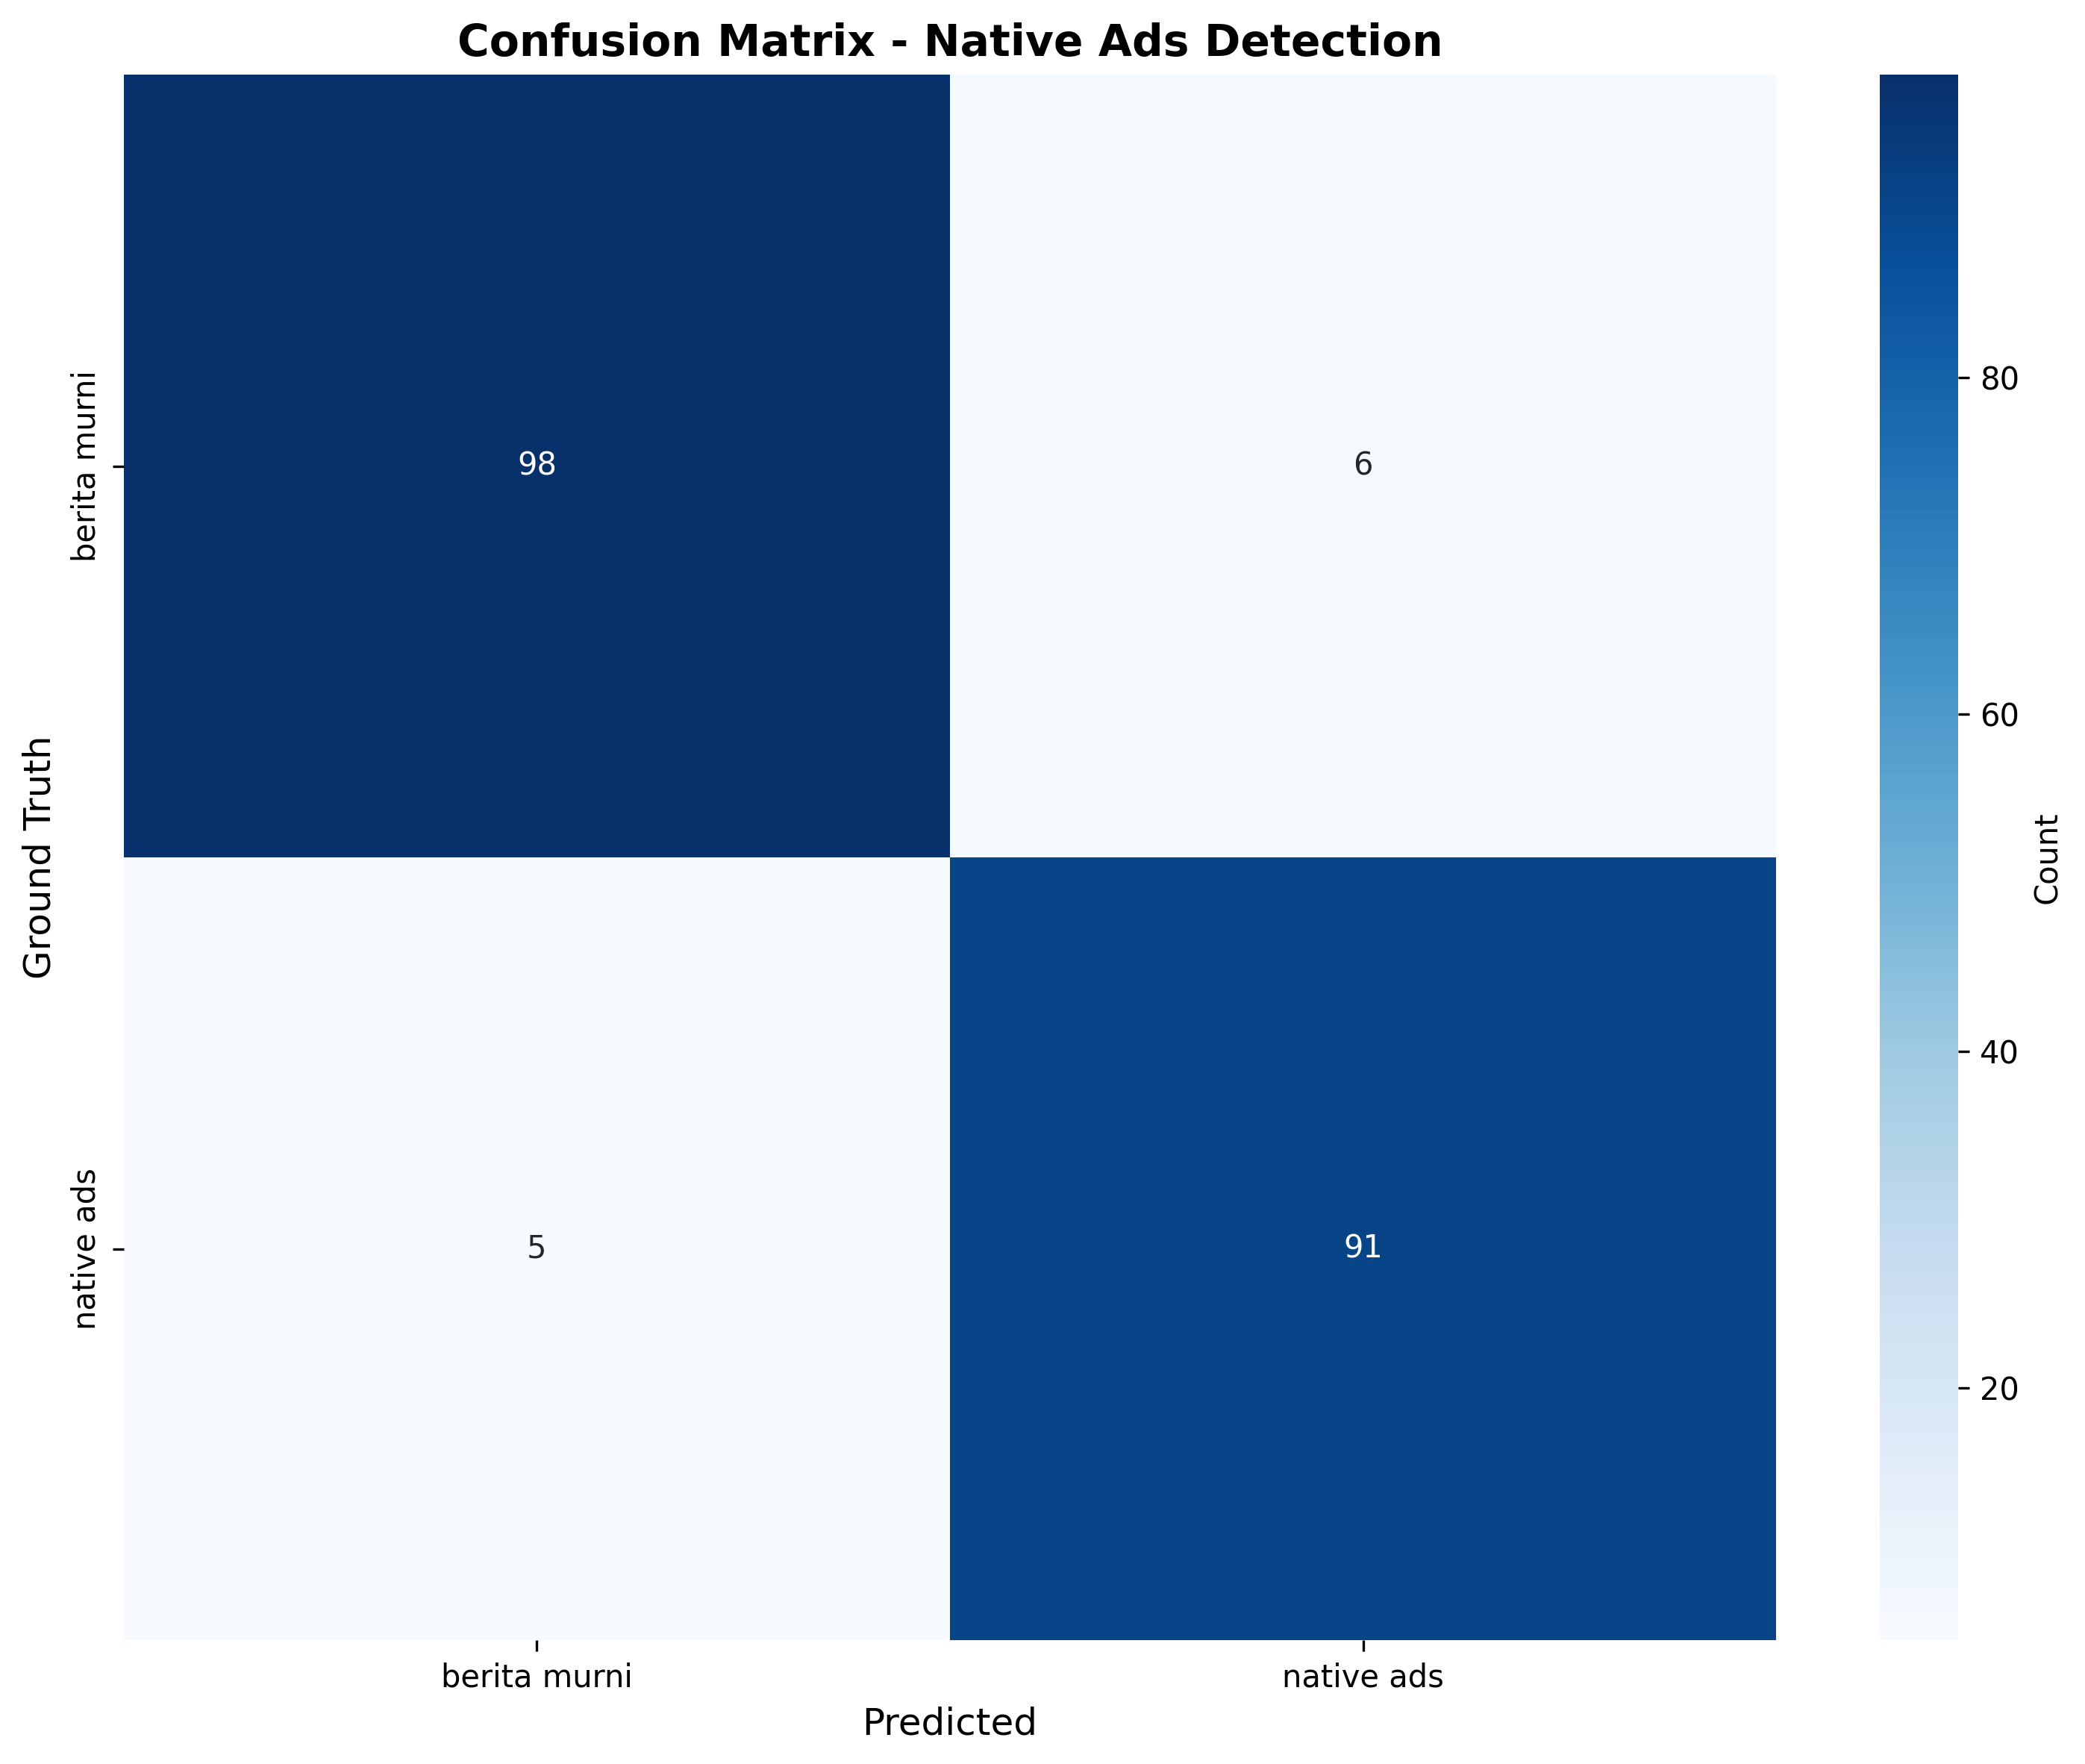
\includegraphics[width=\linewidth]{eval_results/eval_gemma3_12b_native_ads_20260301_043605_confusion_matrix.png}}
\caption{Confusion Matrix untuk AGENA menggunakan Gemma 3 12B.}
\label{fig:confusion_matrix}
\end{figure}


\section{Diskusi}
\label{sec:discussion}
Hasil ini memvalidasi hipotesis inti AGENA: bahwa mendekomposisi deteksi iklan \textit{native} ke dalam \textit{pipeline} multi-agen dengan penalaran berbasis RAG menghasilkan peningkatan terukur dibandingkan klasifikasi statis, baik dalam akurasi maupun interpretabilitas keluaran.

\subsection{Analisis Hard Negatives}
Sumber kesalahan klasifikasi yang konsisten di semua model yang diuji adalah kategori \textit{Hard Negative}. Ini adalah artikel berita yang akurat secara faktual yang menyebutkan entitas perusahaan, produk, atau program pemerintah tanpa niat promosi. Sebagai contoh, pelaporan infrastruktur rutin menyebut kontraktor swasta, dan \textit{Classifier Agent} AGENA terkadang menandai ini berdasarkan pola kata kunci daripada konteks naratif. Bias ``pemicu-merek'' ini lebih menonjol pada model Qwen dan Llama dibandingkan Gemma 3 12B. Mengatasi hal ini di penelitian mendatang memerlukan perluasan basis pengetahuan dengan proporsi yang lebih besar dari contoh \textit{Hard Negative} untuk meningkatkan diskriminasi negatif.

\subsection{Peran Explainer Agent dalam Integritas Jurnalistik}
Kontribusi praktis AGENA adalah \textit{Explanation Agent}, yang menghasilkan justifikasi tingkat-artikel yang dapat ditinjau editor tanpa memeriksa model secara internal. Untuk setiap klasifikasi, agen memetakan kesimpulannya ke bagian-bagian spesifik artikel melalui alat \texttt{Source\allowbreak Mapper}. Ini menyediakan jalur bukti yang dapat diverifikasi yang mendukung keputusan \textit{override} editorial. Bagi organisasi media yang mempertimbangkan pemantauan konten otomatis, lapisan transparansi ini secara substansial mengurangi hambatan adopsi dibandingkan pengklasifikasi \textit{black-box} \cite{b17}.

\subsection{Implikasi Etis dan Bias Algoritmik}
Klasifikasi konten otomatis pada skala besar memperkenalkan risiko bias sistematis. Gaya pelaporan Indonesia berbeda secara substansial antara portal nasional dan media regional, di mana nada informal dan ekspresi lokal-spesifik dapat menyerupai pembingkaian persuasif secara superfisial. Model yang dilatih terutama pada jurnalisme tingkat nasional mungkin salah menandai gaya pelaporan regional sebagai niat promosi. AGENA sebagian memitigasi ini melalui \textit{RAG grounding} dengan contoh beragam, tetapi studi ini mengakui bahwa evaluasi reguler untuk bias linguistik regional diperlukan. Kerangka kerja tidak boleh digunakan dalam pengaturan di mana keputusan otomatis memiliki konsekuensi tanpa tinjauan editorial.

\subsection{Pertimbangan Latensi dan Deployment}
\textit{Pipeline} lima agen memerlukan waktu pemrosesan per artikel sekitar 1,5--3 detik. Untuk aplikasi pemantauan \textit{batch}, ini dapat diterima. Untuk aliran \textit{real-time} bervolume tinggi, \textit{deployment} bertingkat mungkin praktis: pengklasifikasi ringan menangani penyaringan rutin, dengan AGENA dipanggil untuk kasus perbatasan atau prioritas tinggi. Implementasi saat ini menargetkan skenario deteksi akurasi-tinggi dan menyediakan tolok ukur untuk pekerjaan optimasi mendatang.

\section{Kesimpulan}
\label{sec:conclusion}
Makalah ini menyajikan AGENA, kerangka kerja AI multi-agen untuk deteksi iklan \textit{native} yang dapat dijelaskan pada berita digital Indonesia. Kerangka kerja ini mengatasi dua keterbatasan utama penelitian sebelumnya: kurangnya interpretabilitas dalam pengklasifikasi berbasis \textit{ensemble}, dan kecenderungan LLM generik untuk berhalusinasi ketika diterapkan pada jurnalisme Indonesia yang domain-spesifik. Dengan menggabungkan basis pengetahuan berbasis RAG dengan strategi \textit{fine-tuning Reasoning-First}, AGENA mencapai akurasi klasifikasi 94,5\% menggunakan Gemma 3 12B sebagai \textit{Classifier Agent} dan menghasilkan jejak penalaran terstruktur yang dapat ditinjau secara editorial.

Studi ablasi mengonfirmasi bahwa setiap komponen \textit{pipeline} berkontribusi pada performa keseluruhan, dengan \textit{Retriever Agent} memberikan peningkatan tunggal terbesar (+12,8\%). Protokol evaluasi \textit{LLM-as-a-Judge} lebih lanjut menunjukkan bahwa akurasi saja merupakan ukuran yang tidak memadai: model kecil yang mencapai akurasi perbatasan melakukannya melalui penalaran dangkal atau hasil halusinasi daripada pemahaman linguistik yang sesungguhnya. Penelitian mendatang akan berfokus pada perluasan basis pengetahuan untuk mencakup lebih banyak contoh \textit{Hard Negative} dari portal berita regional Indonesia, pengurangan latensi per artikel untuk aplikasi \textit{real-time}, dan evaluasi AGENA pada lingkungan berita lintas bahasa.

\begin{thebibliography}{00}
\bibitem{b1} Potdar, M., et al. (2025). Impact of AI on native advertising revenue growth: A review of technological underpinnings and business implications. World Journal of Advanced Engineering Technology and Sciences, 12(01), 180-190.
\bibitem{b2} Seedtag. (2024). The Power of Neuro-Contextual Advertising: Aligning Emotional Context and User Intent. Digital Marketing Reports 2024.
\bibitem{b3} Sahllal, N., \& Souidi, E. M. (2023). A Comparative Analysis of Sampling Techniques for Click-Through Rate Prediction in Native Advertising. IEEE Access, 11, 24511-24526.
\bibitem{b4} Zhou, Z. (2023). Digital Transformation of Advertising: Trends, Strategies, and Evolving User Preferences in Online Advertising. Highlights in Business, Economics and Management, 23, 1224-1229.
\bibitem{b5} Weber, S., et al. (2024). GenAI Advertising: Risks of Personalizing Ads with LLMs. ResearchGate Preprint, September 2024.
\bibitem{b6} Wojdynski, B. W., \& Evans, N. J. (2024). Disclosure and Recognition of Native Advertising in the Age of Generative AI. Journal of Interactive Advertising.
\bibitem{b7} Alshomary, M., et al. (2024). Detecting Generated Native Ads in Conversational Search. Proceedings of the 47th International ACM SIGIR Conference on Research and Development in Information Retrieval, pp. 1024-1033.
\bibitem{b8} Fawaid, J., et al. (2021). Indonesia’s Fake News Detection using Transformer Network. In ACM International Conference Proceeding Series.
\bibitem{b9} Vlad, G.-A., et al. (2019). Sentence-Level Propaganda Detection in News Articles with Transfer Learning and BERT-BiLSTM-Capsule Model. ACL.
\bibitem{b10} Zhang, Y., et al. (2025). Agentic AI: Autonomous Intelligence for Complex Goals: A Comprehensive Survey. IEEE Access, 13, 4521-4545.
\bibitem{b11} Team, Q. (2024). Qwen2.5 Technical Report. Technical Report, Alibaba Group.
\bibitem{b12} Touvron, H., et al. (2023). Llama 2: Open Foundation and Fine-Tuned Chat Models. Technical Report, Meta AI.
\bibitem{b13} OpenAI. (2024). GPT-4o Technical Report. Technical Blog Post.
\bibitem{b14} Rahman, A. F. A., \& Syaifudin, Y. W. (2024). Indonesian Open-Domain Question Answering System using Retrieval-Augmented Generation and Gemma Large Language Model. IEEE Access, 12, 54321--54335.
\bibitem{b15} Brown, T., et al. (2020). Language Models are Few-Shot Learners. In Advances in Neural Information Processing Systems (NeurIPS).
\bibitem{b16} Karras, T., et al. (2024). Analyzing LLM Hallucinations in Retrieval-Augmented Generation for Journalism. Journal of Information Science, Sage.
\bibitem{b17} Darnoto, B. R. P., Siahaan, D., \& Purwitasari, D. (2024). Electronic news dataset for native advertisement detection. Scientific Data, 11(1), 1045. https://doi.org/10.1038/s41597-024-04341-6
\bibitem{b18} Darnoto, B. R. P., Siahaan, D., \& Purwitasari, D. (2023). A Comprehensive Ensemble Deep Learning Method for Identifying Native Advertising in News Articles. In 2023 IEEE 8th International Conference on Software Engineering and Computer Systems (ICSECS), pp. 450--455.
\bibitem{b19} Darnoto, B. R. P., Siahaan, D., \& Purwitasari, D. (2023). SENADA: A Stacked Ensemble Learning for Native Advertisement Detection in Electronic News. IEEE Access, 11, 102341--102355.
\bibitem{b20} Johnson, A., et al. (2024). Explainable AI in Digital Journalism: A Systematic Review of Editorial Requirements. Digital Journalism, Elsevier.
\bibitem{b21} Darnoto, B. R. P., Siahaan, D., \& Purwitasari, D. (2023). Automated Detection of Persuasive Content in Electronic News. Informatics, 10(4), 86. MDPI.
\bibitem{b22} Wang, J., et al. (2025). Real-time Ad Retrieval via LLM-generative Commercial Intention for Sponsored Search Advertising. In Proceedings of the 63rd Annual Meeting of the Association for Computational Linguistics (ACL).
\bibitem{b23} Vaswani, A., et al. (2017). Attention is All You Need. In Advances in Neural Information Processing Systems (NeurIPS).
\bibitem{b24} Choudhary, T. (2025). Political Bias in Large Language Models: A Comparative Analysis of ChatGPT-4, Perplexity, Google Gemini, and Claude. IEEE Access, 13, 11341-11379.
\bibitem{b25} Lewis, P., et al. (2020). Retrieval-Augmented Generation for Knowledge-Intensive NLP Tasks. In Advances in Neural Information Processing Systems (NeurIPS).
\bibitem{b26} Pinecone. (2024). Scaling Vector Search to Billions of Embeddings for Enterprise RAG. White paper.
\bibitem{b27} Milvus Team. (2025). Vector Database Benchmarks for News Recommendation and Deceptive Content Detection. Zilliz Research Reports.
\bibitem{b28} Sharma, V., et al. (2025). Empowering Text Classification with Agentic AI: A Systematic Review. In 2025 International Conference on Artificial Intelligence and Machine Vision (AIMV).
\bibitem{b29} Han, J., et al. (2024). Agentic Workflow: Rethinking Multi-Agent Collaboration for Complex Reasoning. IEEE Transactions on Neural Networks and Learning Systems.
\bibitem{b30} Wu, Q., et al. (2023). AutoGen: Enabling Next-Generation LLM Applications via Multi-Agent Conversation. International Conference on Learning Representations (ICLR).
\bibitem{b31} Gautam, A. (2025). Multi-agent Systems for Misinformation Lifecycle: Detection, Correction And Source Identification. Technical Report, Indiana University.
\bibitem{b32} Valchanov, D. (2025). Enhancing Fake News Detection using Multi-Agent LLM Frameworks. Master's Thesis, RWTH Aachen University.
\bibitem{b33} Purwitasari, D., et al. (2024). A Systematic Review on Semantic Role Labeling for Information Extraction in Low-Resource Data. IEEE Access, 12, 12345--12356.
\bibitem{b34} Purwitasari, D., et al. (2025). Dangerous Speech Classification on Twitter Using Multilabel Aspects and Structural Features. IEEE Access, 13, 5678--5689.
\bibitem{b35} Siahaan, D., et al. (2025). Graph-Based Module Clustering Using Machine Learning Model in Object Oriented Software. IEEE Access, 13, 2134--2145.
\bibitem{b36} Hu, E. J., et al. (2021). LoRA: Low-Rank Adaptation of Large Language Models. International Conference on Learning Representations (ICLR).
\bibitem{b37} Dao, T. (2023). FlashAttention-2: Faster Attention with Better Parallelism and Work Partitioning. International Conference on Learning Representations (ICLR).
\bibitem{b38} Smith, K., et al. (2023). The Ethics of Native Advertising in the Age of Generative AI. Journal of Media Ethics, Taylor \& Francis.
\bibitem{b39} Devlin, J., et al. (2018). BERT: Pre-training of Deep Bidirectional Transformers for Language Understanding. Proceedings of the 2019 Conference of the North American Chapter of the Association for Computational Linguistics.
\bibitem{b40} Team, G. (2024). Gemma 2: Improving Open Language Models via Multistage Distillation. Technical Report, Google DeepMind.
\bibitem{b41} Wijaya, H., et al. (2024). LORAXBENCH: A Multilingual Reasoning Benchmark for Indonesian Regional Languages. ACL Anthology.
\bibitem{b42} Pratama, A., et al. (2024). IndoCareer: Evaluating LLMs on Indonesian Professional Certification Exams. Proceedings of the 62nd Annual Meeting of the Association for Computational Linguistics.
\bibitem{b43} Sari, N., et al. (2024). IndoMMLU: An Indonesian Massive Multitask Language Understanding Benchmark. In Proceedings of the 2024 Conference on Empirical Methods in Natural Language Processing.
\bibitem{b44} Gunawan, E., et al. (2024). IndoCulture: Cultural Reasoning across Indonesian Provinces for Large Language Models. NeurIPS 2024 Workshop.
\bibitem{b45} Artificial Analysis. (2025). Multilingual Index: Indonesian Language Reasoning Scores. Technical Report.
\bibitem{b46} Chen, X., et al. (2024). AdvAD: Exploring Non-Parametric Diffusion for Imperceptible Adversarial Attacks on Text Classifiers. NeurIPS 2024.
\bibitem{b47} IEEE Computer Society. (2026). Special Issue: Fighting Fake: Disinformation and Misinformation. IEEE Computer, July 2026.
\bibitem{b48} Darnoto, B. R. P., Siahaan, D., \& Purwitasari, D. (2022). A Novel Framework to Detect Irrelevant Software Requirements Based on MultiPhiLDA as the Topic Model. Informatics, 9(3), 67. MDPI.
\end{thebibliography}

\begin{IEEEbiography}[{
\includegraphics[width=1in,height=1.25in,clip,keepaspectratio]{brian.jpg}}]{Brian Rizqi Paradisiaca Darnoto} menerima gelar master di bidang informatika dari Institut Teknologi Sepuluh Nopember, Surabaya, Indonesia, pada tahun 2022, di mana ia saat ini sedang menempuh studi Doktoral. Ia juga merupakan Dosen di Universitas Jember, Indonesia. Minat penelitiannya meliputi kecerdasan buatan, pemrosesan bahasa alami, dan rekayasa perangkat lunak.
\end{IEEEbiography}

\begin{IEEEbiography}[{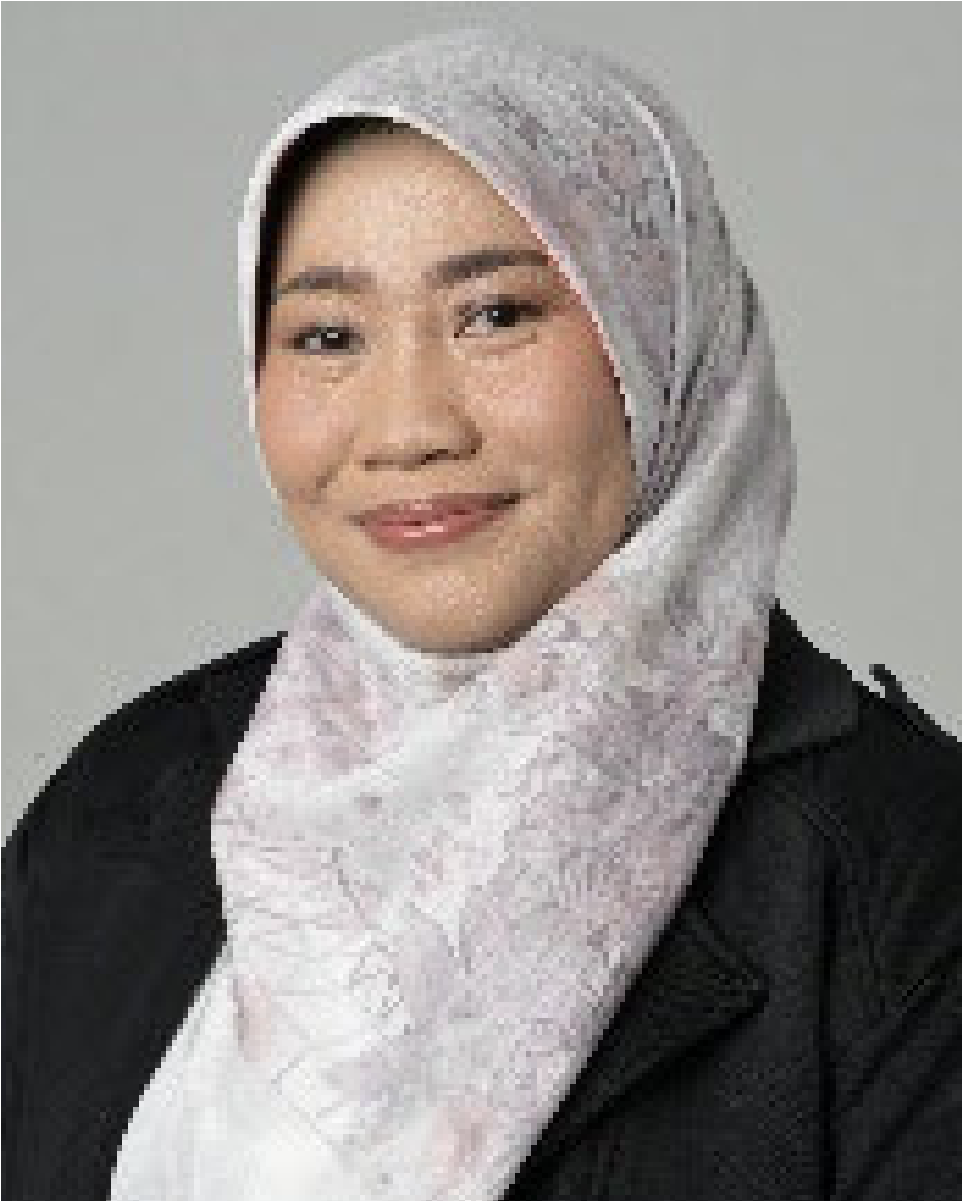
\includegraphics[width=1in,height=1.25in,clip,keepaspectratio]{diana.png}}]{Diana Purwitasari} (Senior Member, IEEE) adalah seorang Profesor di Departemen Informatika, Institut Teknologi Sepuluh Nopember. Minat penelitian beliau meliputi \textit{information retrieval}, \textit{social network analysis}, dan \textit{web mining}.
\end{IEEEbiography}

\begin{IEEEbiography}[{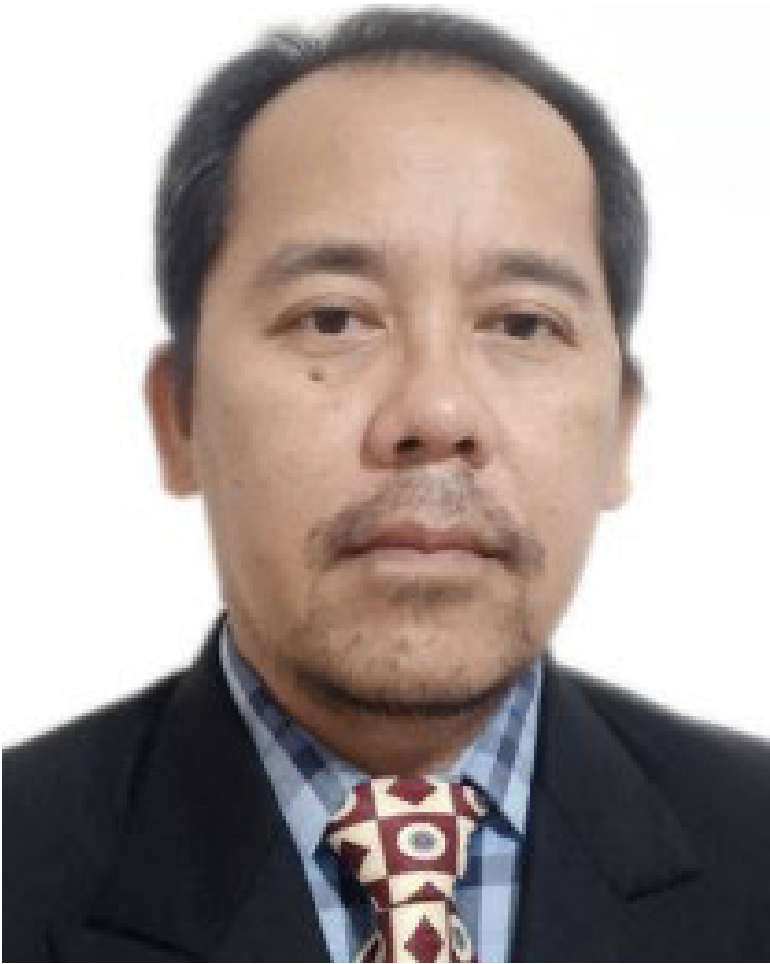
\includegraphics[width=1in,height=1.25in,clip,keepaspectratio]{daniel.png}}]{Daniel Oranova Siahaan} (Member, IEEE) adalah seorang profesor di Departemen Informatika, Institut Teknologi Sepuluh Nopember. Beliau telah menerbitkan lebih dari 50 artikel jurnal dan makalah konferensi mengenai rekayasa perangkat lunak. Minat penelitiannya meliputi rekayasa peranti pemenuhan kebutuhan (\textit{requirements engineering}) dan pemrosesan bahasa alami.
\end{IEEEbiography}

\EOD
\end{document}
